%%%%%%%%%%%%%%%%%%%%%%%%%%%%%%%%%%%%%%%%%%%%%%%%%%%%%%%%%%%%
%%% Based on LaPreprint: PREPRINT TEMPLATE
%%% Source: https://github.com/roaldarbol/LaPreprint/tree/b32e34b797298ed151e979e0871b36ec06108110
%%%%%%%%%%%%%%%%%%%%%%%%%%%%%%%%%%%%%%%%%%%%%%%%%%%%%%%%%%%%


% Declare document class
\documentclass[9pt,biorxiv,lineno,onehalfspacing]{lapreprint}
% Choose between "biorxiv", "medrxiv", "arxiv" and "chemrxiv". Otherwise defaults "Preprint".
% Choose between "blue" and "red" colour scheme. Defaults to "blue".
% Use the "onehalfspacing" option for 1.5 line spacing.
% Use the "doublespacing" option for 2.0 line spacing.
% Use the "lineno" option for line numbers.
% Use the "endfloat" option to place floats after the bibliography.

% Import packages
\usepackage{pdflscape}  % For putting pages in landscape mode
\usepackage{rotating}   % For rotating specific elements
\usepackage{textgreek}  % Greek symbols
\usepackage{gensymb}    % Symbols
\usepackage[misc]{ifsym} % For the \Letter symbol
\usepackage{orcidlink}  % For the \orcidlink
\usepackage{listings}   % For inserting code chunks
\lstset{
basicstyle=\small\ttfamily,
columns=flexible,
breaklines=true
}
\usepackage{colortbl}   % For Knitr table colouring
\usepackage{tabularx}   % For making Knitr tables compatible
\usepackage{longtable}  % For multi-page tables
\usepackage[labelformat=simple]{subcaption}
\usepackage{multirow}
\usepackage{snotez}     % For sidenote environments. enotez for endnotes
\usepackage{csquotes}   % For language-based quote rules (helps BiBLaTeX)

%\usepackage[table,xcdraw]{xcolor}
\usepackage[utf8]{inputenc}
%\usepackage[all]{hypcap}
\usepackage{microtype} %makes text formatting slightly more readable
\usepackage{libertine} %uses open source font
\usepackage{svg}
\usepackage{authblk}
\usepackage[labelfont=bf]{caption}
\usepackage{adjustbox}
\usepackage{pgffor}

% for annotated equations
\usepackage{annotate-equations}
\usepackage{amsmath}
%\usepackage{amssymb}
\usepackage{mathtools}
\usepackage{tikz}
\usetikzlibrary{backgrounds}
\usetikzlibrary{arrows,shapes}
\usetikzlibrary{tikzmark} % for \tikzmarknode
\usetikzlibrary{calc} % for computing the midpoint between two nodes, e.g. at ($(p1.north)!0.5!(p2.north)$) 
\newcommand{\highlight}[2]{\colorbox{#1!17}{$#2$}}
\newcommand{\highlightdark}[2]{\colorbox{#1!47}{$#2$}}
\newcommand\ttiny{\fontsize{4}{5}\selectfont}
\newcommand\tttiny{\fontsize{2}{3}\selectfont}

\hypersetup{
  colorlinks   = true, %Colours links instead of ugly boxes
  urlcolor     = blue, %Colour for external hyperlinks
  linkcolor    = gray, %Colour of internal links
  citecolor    = gray  %Colour of citations
}

%%%%%%%%%%%%%%%%%%%%%%%%%%%%%%%%%%%%%%%%%%%%%%%%%%%%%%%%%%%%
%%% BIBLIOGRAPHY
%%%%%%%%%%%%%%%%%%%%%%%%%%%%%%%%%%%%%%%%%%%%%%%%%%%%%%%%%%%%
\usepackage[			% use biblatex for bibliography
	backend=biber,      % use biber or bibtex backend
    style=numeric-comp,   % choose style
	natbib=true,		% allow natbib commands
	hyperref=true,	    % activate hyperref support
	alldates=year,      % only show year (not month)
    uniquename=false,   % don't add firstnames when citing multiple sources by the same author
    maxbibnames=12,     % maximum number of author names to list in bibliography before 'et al' is used instead
    sorting=none,       % sort by order of appearance
]{biblatex}

\AtEveryBibitem{
    \clearfield{urlyear}
    \clearfield{urlmonth}
    \clearlist{language}
    \clearfield{url}
    \clearfield{note}
   % \clearfield{issn}
}

% Update to your bibliography file
\addbibresource{bib.bib}
\addbibresource{Dec2023-Converted.bib}


%%%%%%%%%%%%%%%%%%%%%%%%%%%%%%%%%%%%%%%%%%%%%%%%%%%%%%%%%%%%
%%% ARTICLE SETUP
%%%%%%%%%%%%%%%%%%%%%%%%%%%%%%%%%%%%%%%%%%%%%%%%%%%%%%%%%%%%

% Paper title
\title{The origin of color categories}

\author[ \orcidlink{0000-0002-4579-003X} 1 \Letter]{Daniel J. Garside}
\author[ \orcidlink{0000-0002-2532-9780} 1,2]{Audrey L.Y. Chang}
\author[ \orcidlink{0000-0003-1570-9576} 1]{Hannah M. Selwyn}
\author[ \orcidlink{0000-0001-7715-9253} 1,3 \Letter]{Bevil R. Conway}

% Affiliations
\affil[1]{Laboratory of Sensorimotor Research, National Eye Institute, National Institutes of Health}
\affil[2]{present address: Vilcek Institute of Graduate Biomedical Sciences, New York University}
\affil[3]{National Institute of Mental Health}

% Other metadata. Feel free to add your own
\metadata[]{\Letter\hspace{.5ex} For correspondence}{ \href{mailto:danny.garside@nih.gov}{danny.garside@nih.gov} or \href{mailto:bevil@nih.gov}{bevil@nih.gov}}

%\metadata[\authfn{1}\authfn{2}\authfn{3}]{}{Here's a few symbols to denote contribution specifics, e.g. authors who contributed equally to the work.} %!!!!!!!!!!!!!
%\metadata[]{Present address}{49 Convent Drive, Bethesda, MD-20892-4435, USA} 
% \metadata[]{Data availability}{Data availability statement. 
% Preprocessed data could be available e.g. on \href{https://zenodo.org/}{Zenodo}.} %!!!!!!!!!!!!!!!!
\metadata[]{Data availability statement}{All data and code are available on \href{https://github.com/NEI-LSR/MacaqueColorCategories}{github.com/NEI-LSR/MacaqueColorCategories}}
\metadata[]{Code availability statement}{All data and code are available on \href{https://github.com/NEI-LSR/MacaqueColorCategories}{github.com/NEI-LSR/MacaqueColorCategories}}
\metadata[]{Funding}{This research was supported by the Intramural Research Program of the NIH, National Eye Institute.}
\metadata[]{Competing interests}{The authors declare no competing interests.} 

% Surname of the lead author(s) for the running footer
\leadauthor{Garside}
\shorttitle{The origin of color categories}

%%%%%%%%%%%%%%%%%%%%%%%%%%%%%%%%%%%%%%%%%%%%%%%%%%%%%%%%%%%%
%%% ARTICLE START
%%%%%%%%%%%%%%%%%%%%%%%%%%%%%%%%%%%%%%%%%%%%%%%%%%%%%%%%%%%%


\begin{document}
\maketitle
\begin{refsection}

\begin{abstract}

A characteristic feature of the human mind is the use of concepts \citep{carey_origin_2000,tenenbaum_how_2011,RN18739}. A long-standing question is the extent to which concept formation requires language. Here we exploit color as a tool of cognitive science \citep{wilken_detection_2004,zhang_discrete_2008,schurgin_psychophysical_2020} and ask if macaque monkeys have color concepts evident as categories. Color is continuous yet readily categorized, and for humans, color categories express meaning-laden ideas. For example, a ripe strawberry, an embarrassed child, a valentine’s heart, all derive meaning from the concept of redness. Macaques and humans have very similar spectral sensitivity \citep{schnapf_spectral_1987, stoughton_psychophysical_2012, gagin_color-detection_2014} and central visual pathways \citep{lafer-sousa_color-biased_2016}, yet for our purposes they usefully lack language. Whether macaques have consensus color categories is unresolved \citep{sandell_color_1979,fagot_cross-species_2006,siuda-krzywicka_biological_2019}, but if they do, then language cannot be required. Alternatively, if macaques do not have color categories, then color categories are probably not innate. We tested macaques by adapting a match-to-sample paradigm used in humans to uncover color categories from errors in matches \citep{bae_why_2015}. When analyzed with the same methods used previously \citep{bae_why_2015,zhang_discrete_2008}, data in macaques showed evidence for two consensus color categories, not four as in humans. Individual macaques showed additional private color categories, indicating that the capacity to form categories does not depend on language. Further analysis with a newer approach \citep{schurgin_psychophysical_2020} shows that the evidence for the two consensus color categories could be explained by an unwitting non-uniformity in the presumed uniform color space, without invoking cognitive mechanisms. These results show that macaques do not have consensus color categories, they suggest that color categories are not innate, and they allow us to reverse-engineer a perceptually uniform color space that is unconfounded by language.  

\end{abstract}

%\section{Introduction}
This is just a test document for illustrative purposes.

%\section{Results}
\begin{figure}
    \begin{fullwidth}
    \centering
    \includegraphics[width=\textwidth+4cm,trim={0 20cm 0 0},clip]{../Figures/flat/F2_CombinedMMResults_5.jpg}
    \caption{\textbf{Macaque monkeys appear to show two consensus color categories when the data are analyzed with a mixture model that computes the average distribution of the choices for each cue.}
	\textbf{a}, Psychometric functions for the four animals showing the accuracy of the matches as a function of the difference in hue angle between the cue and the foil that is closest in color to the cue. 
	The easiest trials were defined as those where the foil color nearest to the cue color were almost on the opposite side of the color circle. See SI Figure 2 for 95\% CI. 
	\textbf{b}, Mixture model results averaged across the four animals. The data were subsampled so that the same number of completed trials for each animal (24526) were included in the analysis. Error shading shows 95 \%CI. 
	The data recover two significant negative-slope zero-crossings (black dots), corresponding to two color categories. 
	\textbf{c}, Polar plot of the results in (b) with the zero crossings of the negative slope (following the trace counterclockwise) again indicated by black dots. The angle of the two inferred color categories [95 \% C.I.] are 13 [6, 20] (a peach color) and 211 [206, 216] (a teal color). }
    \label{fig:AvResults}
    \end{fullwidth}
\end{figure}

The four animals performed well on the task, achieving a lapse rate of 7\%, 7.1\%, 5.8\%, 14.3\% (Figure 2a; the plots of individual animals showing 95\% CI are provided in SI Figure 1). The results averaged across the four animals, analyzed using the mixture model as used previously to analyze data collected in humans \citep{bae_why_2015,zhang_discrete_2008} (see Methods), provided clear evidence of choice biases (Figure 2). But the consensus color categories inferred using this analysis do not support any of the predictions: the animals appeared to show two consensus color categories, not four as in humans. To the extent that the macaque is an accurate model of the human, these results show that the four color categories manifest in humans are not innate. The centers of the two apparent consensus color categories recovered in the monkeys were at angle 13 (a peach color) and 211 (a teal color). All four animals showed evidence of these two color categories (SI Figure 4).

\paragraph{Two possible explanations for choice biases in macaque monkeys}

\begin{figure}
    \begin{fullwidth}
    \centering
    \includegraphics[width=\textwidth+4cm,trim={0 7cm 0 0},clip]{../Figures/flat/F3_TCCModel_6.jpg}
    \caption{\textbf{Behavioral data showing that putative color categories in macaque monkey can be explained by stimulus-space non-uniformities.} \textbf{a}, Color matches made by an agent with a cognitive color category, using a paradigm with stimuli that uniformly sample a truly uniform underlying perceptual color space (gray circle). 
	The distribution of matches comprises a similarity function (turquoise Gaussian) that is symmetric but with a peak deviated towards the category center. 
	\textbf{b}, Color matches made by an agent lacking cognitive color categories, using a paradigm with stimuli that non-uniformly sample a truly uniform underlying perceptual color space (gray circle). 
	The distribution of matches comprises a similarity function (turquoise asymmetric Gaussian) that is biased towards the more densely sampled region of the color space. 
	The bias arises simply because there are more choice options close to the cue color counterclockwise to the cue. 
	Note that in both a and b, the average of the distribution of matches is similarly deviated counterclockwise to the cue although the similarity functions differ. 
	\textbf{c}, Mixture-model analysis of a simulated data set with a cognitive bias. 
	\textbf{d}, Mixture-model analysis of a simulated data set with a stimulus space non-uniformity. 
	\textbf{e, f}, Similarity matrix for the same simulated data set analyzed in panel c, d. The axes depict the colors uniformly sampling CIELUV. The turquoise-colored traces shows the similarity functions for the cue in a,b.}
    \label{fig:TCCDemo}
    \end{fullwidth}
\end{figure}

The colors we used were defined by the International Commission on Illumination (CIE) to be approximately perceptually uniform. 
But it has long been recognized that there may be non-uniformities in the space \citep{stockman_colorimetry_2010}, although it has not been clear how to test for them; some have argued that perceptual uniformity may be task-dependent or simply unattainable \citep{judd_ideal_1969}. One might even suppose that if language influences color perception, as stipulated by the Sapir-Whorf hypothesis, then all color spaces generated by human observers could be shaped by language. Could the macaque consensus color categories be attributed not to a true cognitive category (Figure 3a) but to unrecognized distortions in the presumed uniform space of colors (Figure 3B)?
Both explanations could introduce biases in the distribution of matches.

The difference in the two explanations can be understood by considering the relationship between two neighboring colors. 
For the cognitive-bias account, there is an asymmetry between the colors if there is a category center nearby.
The color further from the category center will be more likely mistaken for the color closer to the category center than the other way around. 
Whereas for the non-uniform color space, there is no asymmetry in mismatches between neighboring colors. 
These two explanations would produce different shaped distributions of matches: the cognitive bias would yield the same width distribution for all cues around the color circle, but the peak of the distribution would deviate from the cue to varying degrees depending on the proximity of the cue to the category center. 
A stimulus space non-uniformity, meanwhile, would yield an asymmetric distribution that varies in width depending on sampling density of the underlying uniform color space, with regions that are relatively densely sampled having broader distributions. 
We refer to the distributions of matches for a cue, plotted in CIELUV, as its similarity function (hypothetical similarity functions shown in turquoise in Figure 3e and 3f).

To illustrate that the behavioral data could be explained by either a cognitive-bias account or a stimulus-space non-uniformity, we generated two sets of simulated data. 
One data set was generated with a simulation that used a uniform space and a bias arising from cognitive categories, and the other data set was generated with a simulation that used non-uniform sampling of an underlying uniform color space and no cognitive categories.
The data sets from both simulations gave rise to the same pattern of results when analyzed with a mixture model (Figure 3e and 3f).
These simulated data sets were chosen for illustration purposes because they correspond to the pattern of behavioral results (compare the simulated results with Figure 2c). 
The simulations show that the results recovered by the mixture model could be explained by stimulus space non-uniformities without appeal to cognitive color categories. 

To tease apart the possible underlying causes of the behavioral results, we extended the Target Confusability Competition (TCC) model \citep{schurgin_psychophysical_2020} (see Methods). 
The standard implementation of the TCC model assumes the same similarity function for each color. 
The extended version developed presently allows the similarity function to vary as a function of color. To distinguish the extended version of the model from the original, we call it TCC-v, "v" for "vary".
We introduce the concept of a similarity matrix, which captures the set of unique similarity functions for all colors in the space.
Let's consider three versions of the TCC-v model.
The simplest (“null”) model has the same two-parameter similarity function for each color, centered on the target color (this is conceptually equivalent to the original TCC model).  
The "cognitive bias" version of the model specifies similarity functions for each color with peaks that can deviate from the target color (Figure 3a). 
The result is a similarity matrix that has a band of constant width along the inverse diagonal but deviates to one side at color-category locations in the color space. 
The "stimulus-space non-uniformity" version of the model, meanwhile, has a similarity function for each target color that fixes the peak to the target color but where the angular distances between the colors can differ for different colors (Figure 3f). 
This results in a similarity matrix that is symmetric about the inverse diagonal, but which bulges out away from the diagonal at locations in the color space that are oversampled. 
The shape of the distribution of matches for a cue near the zero-crossing of the negative slope in the mixture model is indicated by the turquoise line in the cognitive bias and stimulus space non-uniformity versions of the TCC-v model. 
To recap, the similarity matrix in 3e is constructed using the same data as the polar plot in 3c; and the similarity matrix in 3f is constructed using the same data as the polar plot in 3d. 
These results show that different underlying mechanisms could explain the appearance of choice biases in color-matching tasks.

Next, we quantitatively compare the best fitting versions of each model to the behavioral data. 
To facilitate this comparison, we plot the behavioral data with a free-similarity version of the TCC-v model in which every cell in the similarity matrix is an independent model parameter (Figure 4a, 4b; the data for both panels are the same, centered on one or the other of the putative category centers recovered in the mixture model). 
The resulting matrix makes no assumptions about the underlying mechanisms that determine the similarity between any pair of stimuli. 
Now we can ask, are the data illustrated by the free similarity matrix better explained by the stimulus space non-uniformity model or the cognitive bias model? 
In other words, do the panels in Figure 4a and 4b show mirror symmetry with bulges about the diagonal (like Figure 3f) or asymmetry about the diagonal without bulges (like Figure 3e)? By visual inspection, the data are better explained by the stimulus space non-uniformity model, a conclusion affirmed by statistical tests. 

First, the stimulus space non-uniformity model provides a better fit of the data than the null model (Figure 4c). 
Second, the data are better explained by the stimulus-space non-uniformity model than the cognitive bias model (Figure 4d). 
These results strongly suggest that macaque monkeys do not have innate color categories. 
Again, if the macaque is an accurate model of the human, then the results imply that humans do not have innate color categories either. 

The data presented so far are for the four animals combined. 
The individual animals showed some idiosyncratic differences (SI Figure 4).
By mixture-model analysis, one animal showed not only the two consensus choice biases but also a third bias, for pea green (Figure 5a). 
The free similarity matrix for the data from this animal shows an asymmetry about the diagonal at this location in the color space (Figure 5b), showing that this animal has a cognitive bias for pea-green in addition to the consensus biases driven by stimulus-space non-uniformities (free similarity matricies for all animals shown in SI Figure 5). 
These results show that macaque monkeys have the potential to form cognitive color biases, and that the TCC-v model can recover them. The existence of cognitive biases in individual animals is consistent with prior work that observed different patterns of color-matching behavior in two animals using the continuous-matching task that likely reinforces idiosyncratic acquired biases \citep{panichello_error-correcting_2019}.


\begin{figure}
    \begin{fullwidth}
    \centering
    \includegraphics[width=\textwidth+4cm,trim={0 19cm 0 0},clip]{../Figures/flat/F4_TCCResults_3.jpg}
    \caption{\textbf{Similarity matrices for behavioral data averaged across four monkeys show that stimulus-space non-uniformities explain apparent color categories in monkeys.}
    \textbf{a}, Data are centered on the teal-colored category recovered in the mixture model. 
	\textbf{b}, Data are centered on the peach-colored category recovered in the mixture model. 
	\textbf{c}, Negative Log Likelihood (left) and Bayesian Inference Criterion (BIC, right) of the fit of the null model and the stimulus-space non-uniformity model. 
	\textbf{d}, BIC estimates of the fit provided by the stimulus-space non-uniformity model were always lower than BIC estimates of the fit for the cognitive bias model for 100 bootstrap repeats of the analysis (note that the stimulus space non-uniformity model and the cognitive bias model have the same number of parameters). 
	Each data point shows one bootstrap repeat of the analysis. For each boostrap repeat, the number of trials for each animal were the same, set by the animal that completed the smallest total number of completed trials, and that number of trials was drawn with replacement from the total number of completed trials for each animal. 
    } 
    \label{fig:TCCOutput}
    \end{fullwidth}
\end{figure}

\begin{figure}
    \begin{fullwidth}
    \centering
    \includegraphics[width=\textwidth+4cm,trim={0 18cm 0 0},clip]{../Figures/flat/F5_CastorCogBias_6.jpg}
    \caption{\textbf {Color-matching data for one monkey showing evidence for a cognitive color category bias.} 
    \textbf{a}, Mixture-model analysis (same format as Figure 2c). 
	\textbf{b}, Free-similarity matrix (same format as Figure 4a,b) with an asymmetry in the green region indicated by the cross.}
    \label{fig:IndiDataCogBias}
    \end{fullwidth}
\end{figure}

\begin{figure}
    \begin{fullwidth}
    \centering
      \includegraphics[width=\textwidth+4cm,trim={0 15cm 0 0},clip]{../Figures/flat/F6_ColSpace_2}
           \caption{\textbf{Perceptually uniform color space derived from the color-matching data in macaque monkeys.} 
			\textbf{a}, CIELUV color space with 64 color samples at even intervals in hue angle. 
			\textbf{b}, The same color samples plotted in the uniform color space derived from macaque monkeys; note that the axes are not CIELUV but MUCS (macaque uniform color space). 
			\textbf{c}, Colors sampled from evenly from the uniform color space derives from macaque monkeys, projected into CIELUV.}
		\label{fig:MACBEHcolorspace}
    \end{fullwidth}
\end{figure}


\paragraph{A perceptually uniform color space unconfounded by language}

The behavioral data in macaques provide a rare opportunity to reconstruct a perceptually uniform color space unconfounded by language.
We computed, empirically, a transformed color space such that the macaques would, on average, show no choice bias. 
We refer to this space as the Macaque Uniform Color Space (MUCS). 
When colors evenly sampled from the CIELUV space (Figure 6a) are plotted within this macaque-derived uniform color space, colors are bunched around the teal part of the space, and to a lesser extent, around the peach-colored part of the space (Figure 6b). 
We can also take colors sampled at uniform intervals in MUCS and project them into CIELUV (Figure 6c). This arrangement shows relative bunching around the yellows and purples, which correspond to the colors of the poles of the S-cone-opponent axes. 

The mixture-model results in macaque monkeys are strikingly different from those in humans, insofar as the data in humans consistently recover evidence of four consensus categories, while the data in macaque monkeys show evidence of only two consensus categories. But the data in the two species are similar in one regard: they both show repeller points aligned with the poles of the S-cone axis (compare the zero crossings of the positive slopes in Figure 1e with those in Figure 2c) \citep{skelton_biological_2017,bae_why_2015,panichello_error-correcting_2019}. These results raise the possibility that non-uniformities emerge in CIELUV because the contribution of S-cone signals to color perception has not been accurately estimated. Such an inaccuracy may reflect a discrepancy between measurements at threshold (as used in the generation of CIELUV) versus above threshold (as used in the present work), or the amplification of subcortical S-cone signals by the cortex \citep{RN655}.

The present results imply that, contrary to longstanding arguments in empirical philosophy \citep{RN18743}, perception by itself is not sufficient to generate consensus color categories. Meanwhile, prior work has shown that color perception is unnecessary for people to generate rich conceptual knowledge of color, including color categories (congenitally blind people have color concepts) \citep{RN18700}. Taken together, we conclude that color categories are not innate, although color ordering and the capacity to form color categories may be. 

If color categories are not innate, where do they come from? We wonder whether color categories reflect the behavioral relevance of colors in the world; the relevance of things is partially culturally determined, introducing a role for language in shaping consensus color categories. Given that color categories can be learned, as evident in at least one macaque in our study (Figure 5) and two macaques in another study \citep{panichello_error-correcting_2019}, the introduction of language provides a mechanism by which cultures can form consensus about color categories. For example, the parts of scenes labeled as objects by human observers are more likely to be warm colored while backgrounds are more likely to be cool colored \citep{rosenthal_color_2018}, and these statistics predict universal patterns in color naming \citep{gibson_color_2017}. We speculate that the choice biases in humans, which include at least double the number of consensus choice biases in monkeys, likely reflect cognitive biases, and that these cognitive biases achieve consensus through shared behavioral relevance and communication \citep{RN18511,RN18514,RN18602}. 


\section{Discussion}
These results are consistent with those obtained in human infants \citep{skelton_biological_2017} and adults \citep{bae_why_2015,panichello_error-correcting_2019} showing repeller points aligned with the poles of the S-cone axis (the only two repeller points identified in the macaque monkeys aligned with the poles of the S-cone axis, see the zero crossings of the positive slope in Figure 1d,e), and suggest a mechanism by which the non-uniformities emerge in CIELUV. 
The CIELUV colors were defined at threshold, whereas the color-matching experiments were conducted suprathreshold. 
The results in Figure 6c suggest that supra-threshold discrimination for colors that modulate the S-cone axis is higher than at threshold, suggestive of an amplification of subcortical S-cone signals \citep{RN655}. 

The present results are consistent with the idea that color ordering and the capacity to form color categories is innate, but not color categories themselves. 
If color categories are not innate, where do they come from? We wonder whether color categories reflect the behavioral relevance of colors in the world; the relevance of things is partially culturally determined, introducing a role for language in shaping consensus color categories. 
Given that color categories can be learned, as evident in at least one macaque in our study (Figure 5) and two macaques in another study \citep{panichello_error-correcting_2019}, the introduction of language provides a mechanism by which cultures can acquire consensus color categories. 
For example, the parts of scenes labeled as objects by human observers are more likely to be warm colored while backgrounds are more likely to be cool colored \citep{rosenthal_color_2018}, and these statistics predict universal patterns in color naming \citep{gibson_color_2017}. 
We speculate that the choice biases in humans, which include at least double the number of consensus choice biases in monkeys, likely reflect cognitive biases, and that these cognitive biases achieve consensus through shared behavioral relevance and communication \citep{RN18511,RN18514,RN18602}. 


%\section{Conclusion}

\section{Acknowledgments}

Joshua Fuller-Deets adapted code from Shay Ohayon to create the experimental paradigm; Rosa Lafer-Sousa collected pilot data; Whitney Teagle and Shriya Awasthi assisted data collection. 
Funding was provided by the Intramural Research Program of the National Eye Institute. 
We are thankful to the animal care team lead by Denise Parker and Hayden Warnock and to the veterinary staff of the NEI for excellent animal care. 
We thank members of the Laboratory of Sensorimotor Research, attendees of the Colour Group of Great Britain’s January Vision Meeting (2022), the Vision Sciences Society (2022, 2023), the Society for Neuroscience (2023), and the Color Workshop sponsored by the University of Giessen (Summer 2023) for helpful feedback. 
We thank Thorsten Hansen for consultation on color conversions, Ramon Bartolo for mathematical assistance, and Karl Gegenfurtner for the initial prompt to think about testing for color categories in macaques.

\section{Author contributions}

% table? e.g. https://twitter.com/AnneEUrai/status/1361356189284581387
% made previously, Danny didn't have the headspace to show to Bevil: https://github.com/NEI-LSR/MacaqueColorCategories/commit/8b63cd3800d6faa46e5404dd7c43a1fee113a8b5
% 'CRediT' (https://casrai.org/credit/)

Conceptualization: BRC, DJG\newline
Data curation: DJG\newline
Formal Analysis: DJG, HMS, ALYC\newline
Funding acquisition: BRC\newline
Investigation: all authors\newline
Methodology: all authors\newline
Project administration: BRC\newline
Resources: BRC\newline
Software: DJG, HMS, ALYC\newline
Supervision: BRC\newline
Validation: DJG\newline
Visualization: all authors\newline
Writing – original draft: BRC, DJG\newline
Writing – review \& editing: BRC, DJG\newline

\clearpage
\printbibliography[title=Main Text References]
\end{refsection}

% DON'T EDIT. If "endfloat" option is enabled all floats appear before appendices
\if@endfloat\clearpage\processdelayedfloats\clearpage\fi 

\begin{refsection}
\newpage
\section{Methods}
\subsection{Subjects}
Four male rhesus macaques (Macaca mulatta), weighing 8–10 kg% check this!!!
, were implanted with headposts. 
Surgical implantation protocol has been described previously \citep{lafer-sousa_parallel_2013}. % check this!!!
Designation of the subjects are PO, CA, BU, and MO. % this is DG's preference, but open to discussion
All procedures were approved by the Animal Care and Use Committee of the National Eye Institute and complied with the regulations of the National Institutes of Health.
\subsection{Behavioral task}
The animals were trained to perform a 4-Alternative Forced Choice (4-AFC), Delayed Match to Sample task, in which they were shown a colored cue and rewarded for selecting the match option that had the identical color (see \autoref{fig:ParadigmAnalysisPredictions}). 
The colors, described in more detail below, were drawn from a set of 64 colors that evenly sample hue angle of CIELUV color space. 
Each trial was initiated when the animal fixated a small cross at the center of the screen; trials were aborted if the animal did not maintain fixation until the fixation cross disappeared toward the end of the trial. 
Fixation was defined as within a 1.5 degree wide area centered on the fixation cross, well within the precision of the eye tracker.
The trial sequence was as follows. 
Fifty ms after initiating the trial by fixating the central cross, a 3-degree-diameter “cue”  of a color randomly drawn from the set of 64 colors appeared for 750ms. 
The cue was positioned on the monitor at the same location for the whole session on a given day.
From day to day, the center of the cue could vary from 2.5-degrees to 6-degrees eccentricity and be at any angle from fixation.
The cue was followed by a gray screen for a brief “memory” period of 600-900ms, after which four match options appeared along an arc at an eccentricity of 6-degrees. 

The match options had the same shape and size as the cue (3-degree-diameter discs); they were evenly spaced along the arc, with a gap of 2 degrees separating each option. 
The order of the match options on the arc was random. %TODO DG to confirm
In all animals except one (CA), the arc along which the match options were placed was in the visual hemifield opposite to the cue. 
The exact position of the arc within the hemifield varied from trial to trial, so the animals could not anticipate where the choice options would appear. 
Animal CA had a small scotoma spanning ~3degrees of visual angle in a quarter of the visual field as the result of a ~3 mm diameter V1 lesion, so the cue and choices were placed in the same (intact) hemifield, taking care to avoid overlap of the position of the cue and the choices. 


One choice option was always a direct match to the cue, and the other three were randomly sampled without replacement from the remaining 63 stimuli. 
After a random period from 500-1000 ms, the fixation cross disappeared, instructing the monkey to direct its eyes to one of the choices. 
This random period helped guard against the animals making impulsive responses because they could not anticipate when exactly the choice options would appear.
Reward was given only if the animal selected with an eye movement the choice that was identical to the cue. 
If the monkey failed to make a choice within 5 seconds or broke fixation at any point before the termination of the fixation cross, the trial was aborted.

Task difficulty was defined by the set of foil colors that accompanied the direct match for the match options: trials were considered more difficult for smaller differences between the cue color and the foil closest to the cue color. 
The experiment was controlled with custom software written in MATLAB and Psychtoolbox \citep{noauthor_nei-lsrkofiko_2022, kleiner_whats_2007}.

\paragraph{Stimuli}
Stimuli were 3-degree diameter discs presented on a Cambridge Research Systems Display++ screen. 
Colors were defined to be on an equiluminant plane in CIELUV color space, with the luminance matched to the adapting gray background (L* = 76.0693, 38.5cm/m2; adapting field chromaticity was xy\textsubscript{1931}: 0.2684, 0.2409). 
The stimulus set included 64 colors, evenly sampling CIELUV hue angle (5.625-degrees between adjacent stimuli), of equal CIELUV saturation (radius 37), the highest saturation possible for a set of stimuli of equal saturation and luminance given the gamut of the display.
Luminance contrast noise was randomly added to each pixel of the cue and the match options to mitigate chromatic aberration. 
The luminance added to each pixel was updated every frame and drawn uniformly from a continuous range of +/- 5 L* units (the resulting stimulus looks like a colored disc viewed behind a thin veil of television snow). 
CIELUV was used to define the stimuli because it has an associated chromaticity diagram, but the stimuli can readily be transformed into other spaces such as CIELAB and DKL. 

The color stimuli corresponding to the poles of the cone opponent cardinal axes were computed as follows. 
First, the spectra of the stimuli and adapting field were measured using a spectroradiometer. 
These spectra were multiplied by the Smith-Pokorny cone fundamentals to compute the activations for the three classes of cones (LMS), and by the Judd-Vos-modified CIE 2-deg color matching functions to compute luminance. 
The PsychToolbox function “ComputeDKL\_M” was then used to compute a conversion matrix for converting between LMS and cone opponent cardinal axes that define the DKL colorspace. 

\paragraph{Human Data}

Data from published reports using two related tasks completed in human subjects were kindly provided by Gi-Yeul Bae {Bae, 2015 #9761} and Timothy Buschman {Panichello, 2019 #18694}. %!!!!!!!
Both these data sets involved a paradigm in which participants matched the color of a cue to a ring of colors showing a continuous progression of colors around the color circle (a “color wheel”). 
The results of the two prior studies are consistent with each other: when analyzed with a mixture model, both data sets show four color categories corresponding to blue, green, orange, and pink (SI Figure 1); moreover, the results on a version of the task that omits the memory delay period also recover these four color categories {Bae, 2015 #9761}.  %!!!!!!!!!
This prior work shows that the results on the color-matching task are reproducible and robust. 
It is therefore likely that the results of the present version of the task, which is distinguished from the prior work by providing as options discrete targets as opposed to a continuous colored wheel, would also be similar. 
But to test this likelihood, we recruited human participants via Amazon Mechanical Turk to perform the same task used in the macaque monkeys in the present work. 
To request a trial, participants used a mouse to adjust the location of a cursor to click on a fixation cross, after which a cue was shown to one side of the fixation cross, and the cursor disappeared. The cue was displayed for 750 ms. 
After the cue was extinguished, a fixation cross was shown but the cursor remained hidden to de-incentivize mouse movement (1500 ms). Four choices were then shown, and the cursor reappeared; participants made their selection by using the mouse to move the cursor to their choice and clicking the mouse. 
All other aspects of the experimental design were the same as the experiment deployed with the monkeys: 64 colors of equal saturation and luminance (we assumed the monitor that each on-line participant was using matched the sRGB standard), evenly sampling CIELUV. 
The pattern of results was consistent with the published studies using the continuous ring of colors, recovering four significant color categories corresponding to blue, green, orange, and pink (SI Figure 1; see Data Analysis: Mixture Modeling for a description of how these data were analyzed). %!!!!!!
\subsection{Data Analysis}

\paragraph{Mixture Modeling}

To assess the bias in responses for each cue, we computed the distribution of responses on trials where the monkey made an incorrect choice.
For each completed trial, we calculated the error as the angular difference between the correct option and the chosen option.  
For each cue, we computed the number of times the monkey selected each incorrect choice, normalized by the number of times each choice color was available as a choice option for all completed trials of the given cue (though this was approximately uniformly distributed).
We then fit a Gaussian with a variable floor (\autoref{eq:GaussianEquation}) to the error distribution for each cue, using the MATLAB \verb|fit| function with the equation defined as \verb|a*exp(-(((x-b)^2)/(2*c^2)))+d|. 

% demo annotated-equation code from here: https://mirrors.concertpass.com/tex-archive/macros/latex/contrib/annotate-equations/annotate-equations.pdf

%\newpage %Sometimes the annotations don't show up, the hacky solution is to force them onto a new page

\vspace{2em} 
\begin{equation} \label{eq:GaussianEquation}
    \eqnmarkbox[purple]{p1}{a}
    \cdot
    \exp
    -\frac{(x-
    \eqnmarkbox[violet]{b}{b}
    )^2}{2 
    \eqnmarkbox[blue]{c}{c}^2}
    +
    \eqnmarkbox[gray]{d}{d}        
\end{equation}

\annotate[yshift=1em]{above,left}{p1}{height of the curve's peak}
\annotate[yshift=1em]{above}{b}{position of the center of the peak}
\annotate[yshift=-0.75em]{below,left}{c}{standard deviation}
\annotate[yshift=-1em]{below}{d}{floor}
\vspace{2em} 

This fit was weighted by the number of times each choice color was an option for the given cue across all completed trials (though as before, this was approximately uniformly distributed). 
Bias was taken as the difference between the cue and the peak of the corresponding Gaussian, for each cue color ($b$ in \autoref{eq:GaussianEquation}). 
%These values were then smoothed (with a circular moving average filter of 5 cues) since our primary interest was in the broader structure of the bias distribution, and this is shown as the black lines in \autoref{fig:BiasCurves}.
These values, for each stimulus, are plotted as the black lines in \autoref{fig:BiasCurves}.
Where this line falls closer to the center of the figure than the 0$^{\circ}$ line, there is negative bias (which in this representation is counter-clockwise), and vice versa for values above the 0$^{\circ}$ line.
%Attractor points (thought to indicate color category centers) occur where the bias curve crosses the zero line from positive to negative (going counter-clockwise).
%At these points, there is zero bias, and hues on either side provoke choices that are biased inwards towards this point.
%Correspondingly, repeller points occur where the bias curve crosses the zero line from \emph{negative to positive} (again, going counter-clockwise).
%At these points there is also zero bias, but hues either side of this point are biased \emph{away} from this point.
Confidence intervals were extracted from 

%\subparagraph{Confidence intervals}
%To find the 95\% confidence intervals for the locations of the category centers, we performed 1000 bootstraps on all completed trials. For each bootstrapped sample, we found the bias values for each cue color, smoothed the bias curve, and found the category center locations for each bootstrapped dataset. To find the category center locations for the full data set and their confidence interval, we found the category boundaries and segmented all bootstrapped category centers that fell between two consecutive category boundaries. For each of these segments, we found the circular mean and circular standard deviation of all category crossings that fell within these boundaries. 
%\begin{figure}
%\includesvg[inkscapelatex=false, width=\textwidth]{../../Figures/F2_DataAnalysis_v2.svg}
%\caption{\textbf{Task performance.}
%Performance as a function of trial difficulty, quantified as the closeness of the chromatically closest incorrect choice.
%\emph{A.} For one animal, with five example choice sets below for trials where the cue was cue \#28 (correct choice highlighted by dashed line here, not visible to animal).
%\emph{B.} For all animals.
%} 
%\label{fig:TaskPerformance}
%\end{figure}

\paragraph{Target Confusability Competition (TCC)}
A particular disadvantage of the mixture model for our analysis is that we can only use it to analyse the subset of trials where the animal made an incorrect response\footnote{
This is for messy and annoying reasons. 
Firstly, since in our paradigm the choices consist of ``the correct choice'' plus three ``distractors'' (see \nameref{para:4AFC}), the correct choices are greatly over-represented. 
Imagine: by guessing at random, the correct choice would be picked far more frequently than any of the other stimuli, since it is presented on \emph{every trial}, whereas the other stimuli are only presented as distractors with a probability of $\frac{1}{63} + \frac{1}{62} + \frac{1}{62}$. 
This could be normalized out, as we do for the other values, but then a more insidious issue becomes apparent: 
For ``high-error'' choices, the odds of there being a similar choice to that one is less than the odds of there being a similar choice to the ``0-error'' choice, and thus the probability of selecting the correct answer, when normalised, is lower than one would expect. 
%Or to flip the logic: there are slightly higher odds of there being a close distractor to the 0-error stimulus than there is to a high-error stimulus.
You can think of it as: for the high-error choice, there are \emph{2 chances} to pick another choice option that is close to the high-error choice (since one choice is going to be the distant-by-definition 0-error choice), whereas for the 0-error choice there are \emph{3 chances}.
%2 comes from: 1 already used to be the 0-error choice, which by definition is not close to the high-error choice. And 1 is the high error choice itself, so you have 2 left to place.
An additional note for clarity: this is an issue for us because of the sampling required for the AFC paradigm, and is not an issue of concern for those who use a response mechanism where all possible responses are simultaneously presented.
}.
In order to use the full dataset (both incorrect and correct trials), we developed a generative model, based on the \emph{Target Confusability Competition (TCC)} model of \verb|cite{Schurgin+}|.
Using this model, we could use parameter estimation techniques to construct a similarity matrix where each cell represented the similarity between stimulus $s_i$ and stimulus $s_j$. 
Such a similarity matrix is shown in \autoref{fig:SimilarityMatrixPollux} for a single animal (Monkey P).

\begin{figure}
\includegraphics[width=\linewidth]{../../../Figures/working/SimilarityMatrixPollux.png}
\caption{\textbf{Similarity Matrix for Monkey P.}
Similarity between stimulus $s_i$ and stimulus $s_j$, where one is the cue and one is the choice. This is a ``free'' similarity matrix - in that no particular relationship is pre-supposed between any of the stimuli (such as, for example: closer stimuli will be more similar).
%confidence intervals?!?!?! !!!!!!!!!!!!!!
} 
\label{fig:SimilarityMatrixPollux}
\end{figure}


\paragraph{Distinguishing between cognitive biases and non-uniformity of stimulus space}

For these experiments we used a nominally perceptually-uniform colorspace: CIELUV. 
This space has been derived psychophysically, with the goal of minimizing differences in perceptual non-uniformity across the space, for color differences of small magnitudes (the apparent color difference between two points in one part of the space should be equal to the apparent color difference between two points in another part of the space, given that the cartesian distance between the two points in each case be the same).

However, non-uniformities within the space are known to exist (ref?), and uniformity for small color differences does not necessarily assure uniformity for larger color differences (ref? Teunissen?). 
Likewise, uniformity for the conditions under which the psychometric measurements from which the space was determined (considering: spatial, temporal, spectral etc.) does not necessarily assure uniformity across all possible viewing conditions (ref).

With this in mind, it is reasonable to consider what the effect of residual non-uniformity might be on the results of our experiment. 
As discussed by \cite{panichello_error-correcting_2019} (their Figure S5) non-uniformities in colorspace could also potentially lead to systematic biases on tasks such as ours. 
The logic goes as follows: our points are uniformly distributed in our chosen space (\autoref{fig:StimuliAndParadigm}A), but if this space is actually non-uniform compared to the colorspace implicitly being used by an observer, then these same points will be \emph{non}-uniformly distributed in a hypothetical `perfect colorspace'. 
It follows that for each cue color, surrounding distractor points might actually be closer or further away than anticipated. 
If the nearest neighbors on one side of the cue are actually chromatically closer than the neighbors on the other side, one would expect these to be chosen at a higher frequency than the others, creating a systematic bias.

%Unfortunately, these biases act in a similar fashion and are difficult to separate from one another. One potential way to distinguish one type of bias from another is to consider the theoretical relationship between bias and variance: if biases arise due to non-uniformities in colorspace, we would expect the attractor points to also have the \emph{highest} variance in responses. This is because in the hypothetical `perfect space' these points are actually tightly clustered, and so in the presence of noise we can assume that they will be frequently picked over one another. Conversely, at attractor points in spaces where the bias results from categoricality, theory would predict that we would see the \emph{lowest} levels of variance - if these points are conceptualized as `magnets' or `valleys' then we would expect cumulative noise to preferentially return to the attractor point, reducing the variance in responses.



\paragraph{Reconstruction of colorspace}

%\begin{figure}
%\includesvg[inkscapelatex=false, width=\textwidth]{../../Figures/working/Poster_components/BiasCalculation copy.svg}
%\caption{Analysis and Hypotheses.} 
%\label{fig:BiasCalculation}
%\end{figure}


% Amazon Mechanical Turk Data

% Conversion between CIELAB and CIELUV

\paragraph{Discrete vs. Continuous Response Space}
% MechTurk data vs. Bae/Panichello Humans
% Our monkeys vs. Panichello monkeys

\clearpage
\printbibliography[title=Methods References]
\end{refsection}

%%%%%%%%%%%%%%%%%%%%%%%%%%%%%%%%%%%%%%%%%%%%%%%%%%%%%%%%%%%%
%%% SUPPLEMENTARY MATERIAL / APPENDICES
%%%%%%%%%%%%%%%%%%%%%%%%%%%%%%%%%%%%%%%%%%%%%%%%%%%%%%%%%%%%

% modified from: https://tex.stackexchange.com/a/611819/169285
\newcommand{\supplementarysection}{%
  \setcounter{figure}{0}% Reset figure counter
  \let\oldthefigure\thefigure% Capture figure numbering scheme
  \renewcommand{\thefigure}{S\oldthefigure}% 
}

\supplementarysection
\begin{appendixbox}
        \includegraphics[width=\textwidth]{../Figures/flat/SI1_Human.jpg}
        \captionof{figure}{\textbf{foo}
        \emph{a} test
        } 
        \label{fig:Human}
\end{appendixbox}

\begin{appendixbox}
        \includegraphics[width=\textwidth]{../Figures/flat/SI2_psychometric.jpg}
        \captionof{figure}{\textbf{foo}
        \emph{a} test
        } 
        \label{fig:IndiDiff}
\end{appendixbox}

\begin{appendixbox}
        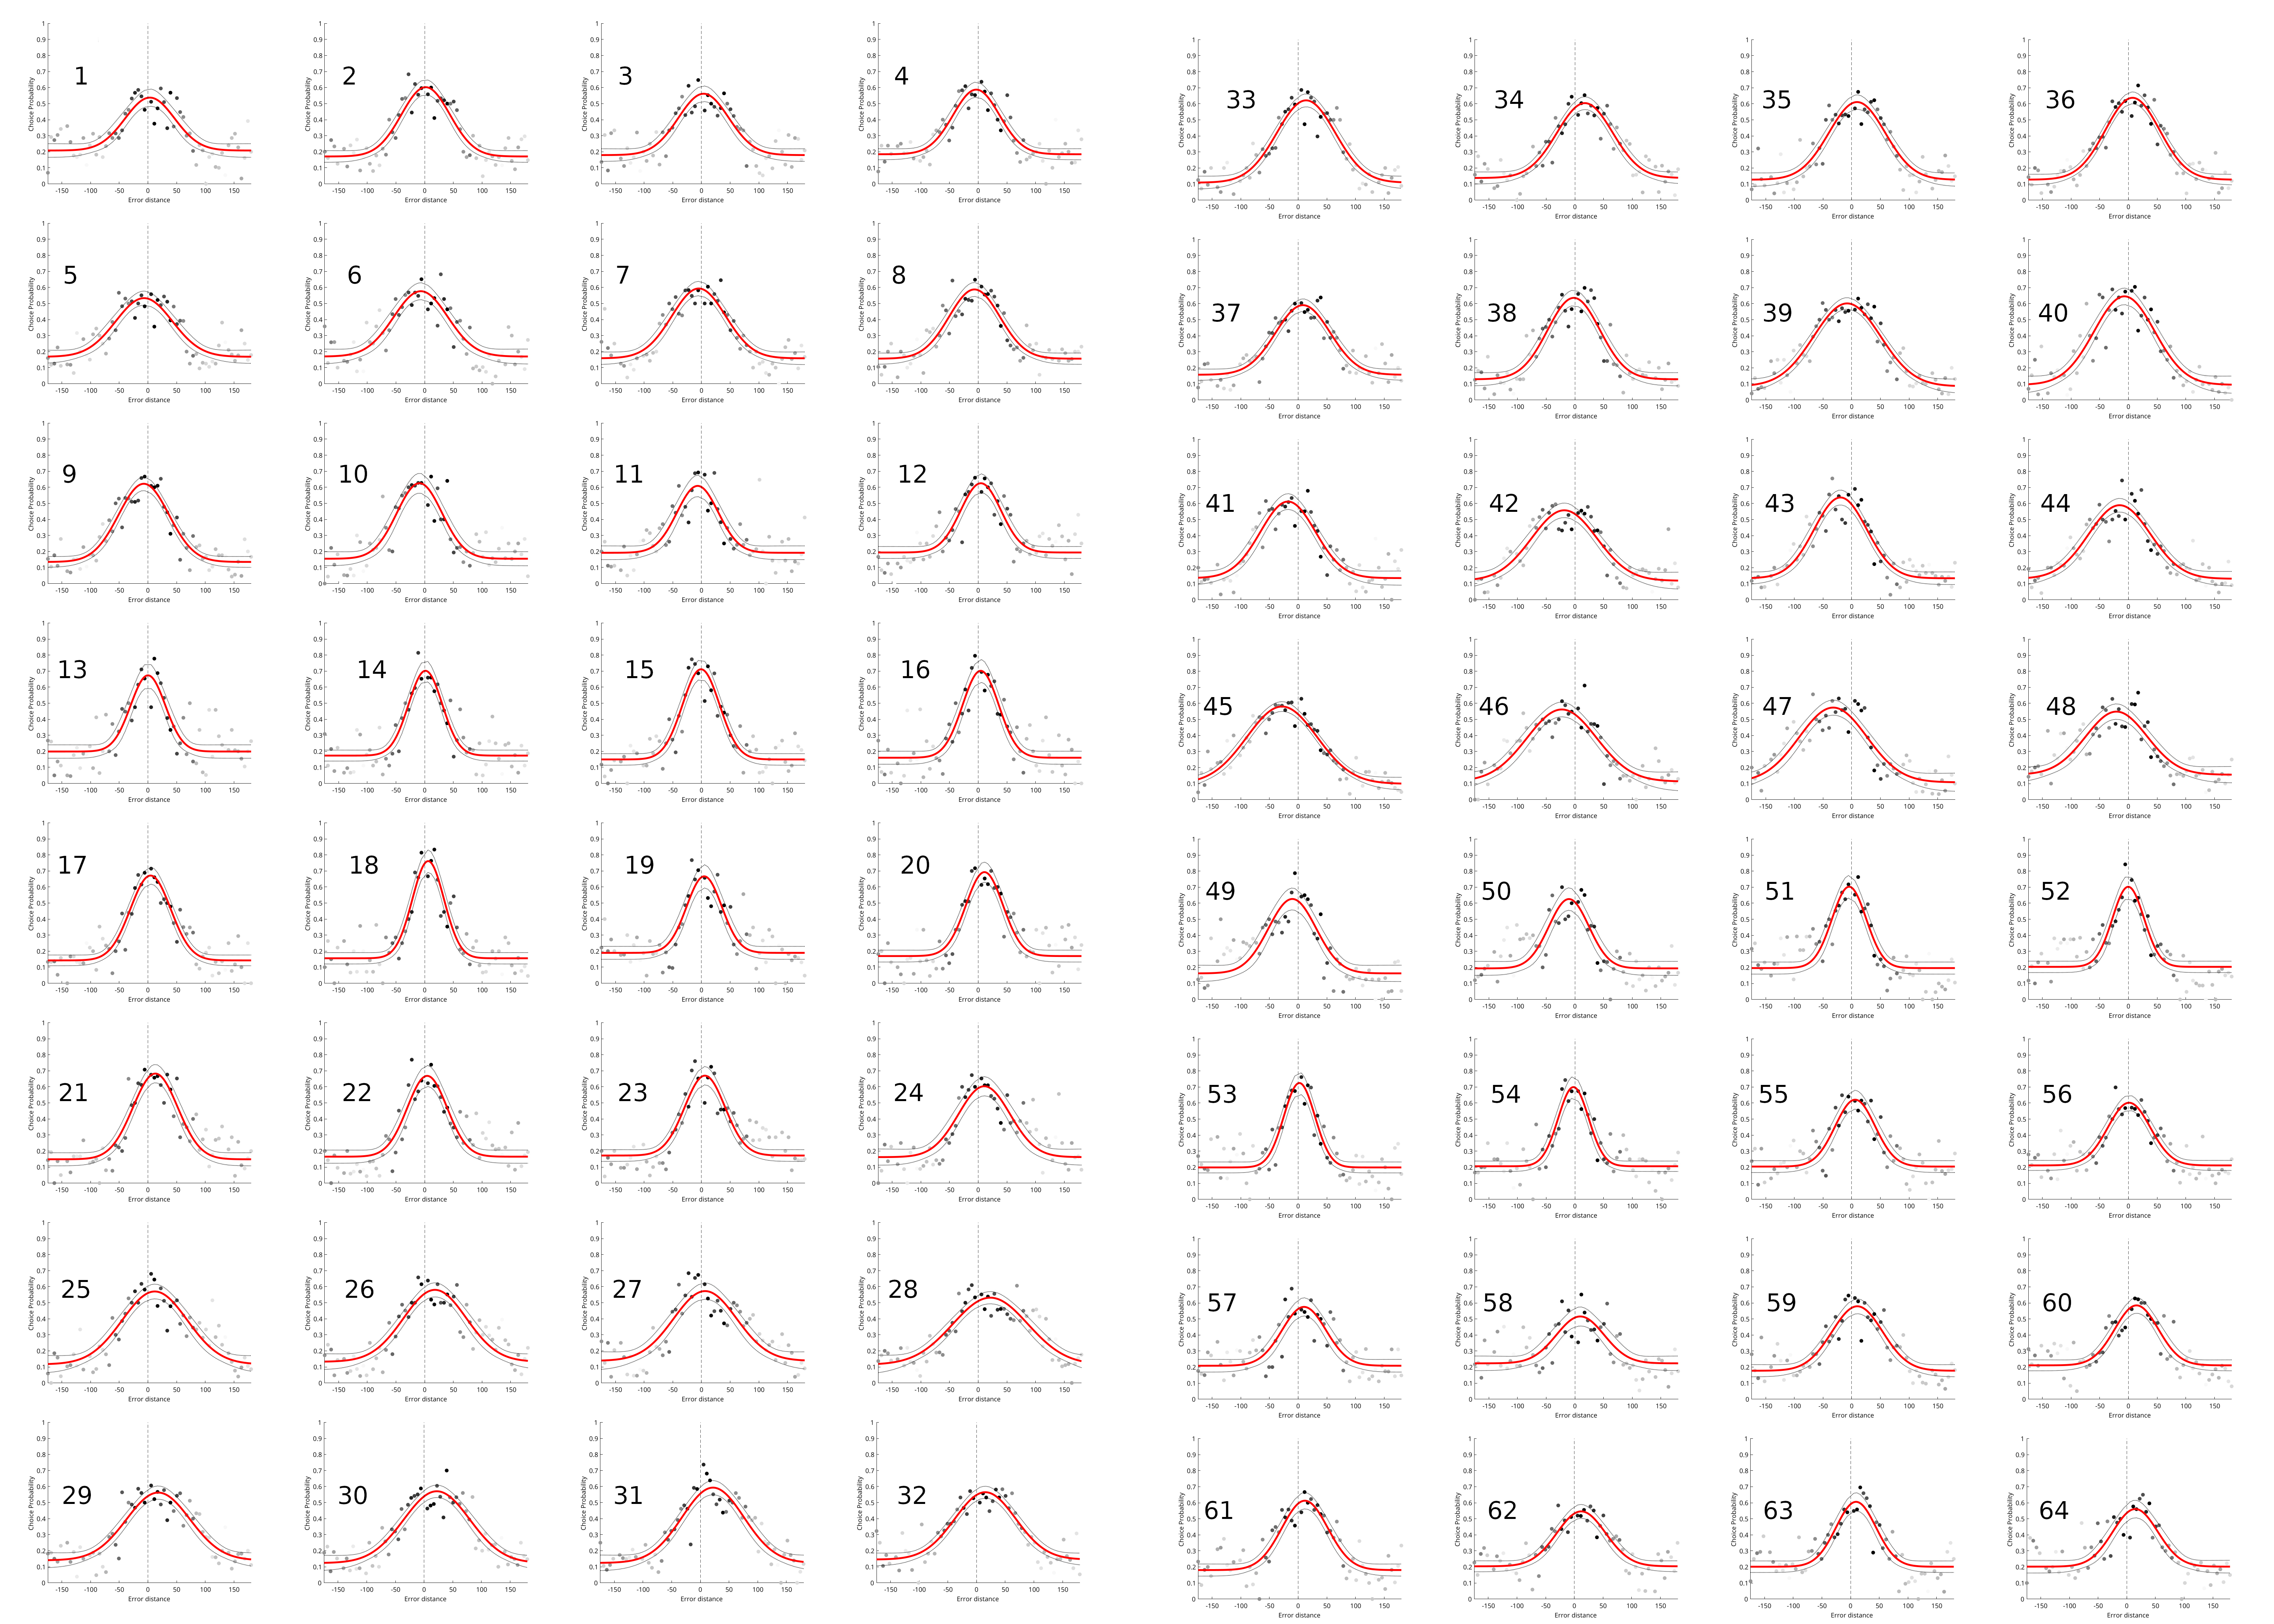
\includegraphics[width=\textwidth]{../Figures/flat/SI3_MMBreakOut.jpg}
        \captionof{figure}{\textbf{foo}
        \emph{a} test
        } 
        \label{fig:MMBreakOut}
\end{appendixbox}

\begin{appendixbox}
        \includegraphics[width=\textwidth]{../Figures/flat/SI4_MM.jpg}
        \captionof{figure}{\textbf{foo}
        \emph{a} test
        } 
        \label{fig:MM}
\end{appendixbox}

\begin{appendixbox}
        \includegraphics[width=\textwidth]{../Figures/flat/SI5_IndTCCv.jpg}
        \captionof{figure}{\textbf{foo}
        \emph{a} test
        } 
        \label{fig:IndiTCC}
\end{appendixbox}

\begin{appendixbox}
        \includegraphics[width=\textwidth]{../Figures/flat/SI6_choiceMatrices.jpg}
        \captionof{figure}{\textbf{foo}
        \emph{a} test
        } 
        \label{fig:choiceProbabilityMatrices}
\end{appendixbox}




%%%%%%%%%%%%%%%%%%%%%%%%%%%%%%%%%%%%%%%%%%%%%%%%%%%%%%%%%%%%
%%% ARTICLE END
%%%%%%%%%%%%%%%%%%%%%%%%%%%%%%%%%%%%%%%%%%%%%%%%%%%%%%%%%%%%

\end{document}




